\documentclass{article}
\usepackage[svgnames]{xcolor}
\usepackage{pgfplots}
\pgfplotsset{compat=1.9}
\begin{document}

\begin{figure}
\centering
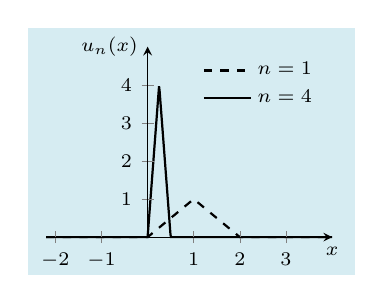
\begin{tikzpicture}
\begin{axis}[width=0.43\textwidth, height=4cm, axis lines=middle, clip=false, axis on top,
             xmin=-2.2, xmax=4, ymin=0, ymax=5, xtick={-2,...,3}, ytick={0,...,4},
             xlabel={$x$}, xlabel style=below, ylabel={$u_n(x)$}, ylabel style=left,
             cycle list={dashed, solid}, every axis/.append style={font=\scriptsize}]
\pgfplotsset{legend style={font=\scriptsize, draw=none, fill=none}}
\addplot[fill=LightBlue!50, draw=none, mark=none, forget plot] % serve solo per lo sfondo colorato
         coordinates {(-2.6,-1) (4.5,-1) (4.5,5.5) (-2.6,5.5)};
\foreach \n in {1,4}
{\addplot+[samples=500, domain=-2.2:4, thick] {\n*max(1-abs(1-\n*x),0)};
   \addlegendentryexpanded{$n=\n$}}
\end{axis}
\end{tikzpicture}

\hspace{0.04\textwidth}

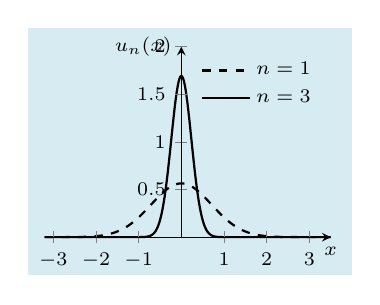
\begin{tikzpicture}
\begin{axis}[width=0.43\textwidth, height=4cm, axis lines=middle, clip=false, axis on top,
             xmin=-3.2, xmax=3.5, ymin=0, ymax=2, xtick={-3,...,3}, ytick={0,0.5,...,1.75},
             xlabel={$x$}, xlabel style=below, ylabel={$u_n(x)$}, ylabel style=left,
             cycle list={dashed, solid}, every axis/.append style={font=\scriptsize}]
\pgfplotsset{legend style={font=\scriptsize, draw=none, fill=none}}
\addplot[fill=LightBlue!50, draw=none, mark=none, forget plot] % serve solo per lo sfondo colorato
        coordinates {(-3.6, -0.4) (4,-0.4) (4,2.2) (-3.6,2.2)};
\foreach \n in {1,3}
{\addplot+[samples=500, domain=-3.2:3.5, thick] {\n*exp(-(\n*x)^2)/sqrt(pi)};
   \addlegendentryexpanded{$n=\n$}}
\end{axis}
\end{tikzpicture}

\end{figure}

\end{document}
